\documentclass{article}

\usepackage[left=2cm,right=2cm, top=2cm, bottom = 2cm]{geometry}
\usepackage{amsfonts}
%%%\usepackage{array}

\usepackage{amsmath}
\usepackage{xcolor}

\usepackage{tikz}
\usepackage{subfigure}

\usepackage{pgfplots}


\pgfplotsset{compat=1.10}
\usepgfplotslibrary{fillbetween}
\usetikzlibrary{patterns}


\pagestyle{empty}

\setlength{\tabcolsep}{15pt}
%%%\renewcommand{\arraystretch}{2.5}

%%%\makeatletter
%%%\newcommand{\thickhline}{%
%%%    \noalign {\ifnum 0=`}\fi \hrule height 2pt
%%%    \futurelet \reserved@a \@xhline
%%%}
%%%\newcolumntype{!}{@{\hskip\tabcolsep\vrule width 2pt\hskip\tabcolsep}}
%%%\makeatother

\newcommand{\deriv}[3][]{\frac{\mathrm{d}^{#1}#2}{\mathrm{d}#3^{#1}}}
\newcommand{\diff}{\;\mathrm{d}}


\begin{document}

\title{Applications of Integration: Arc Length}
\date{}

\maketitle
\thispagestyle{empty}

\Large

\textbf{\underline{Objective: To understand how integration may be used to find the}}

\textbf{\underline{arc length along a curve.}}






\vspace{10mm}



\textbf{Warm-up: Arc Length:}\bigskip

Consider the curve $y=\sqrt{x^2-1}$ for $-1\leq x\leq 1$; this is a semicircle of unit radius---it is the top half of the unit circle, the bottom half being given by the equation $y=-\sqrt{x^2-1}$. We will find the length of this curve; of course, the circumference of a circle is $2\pi r$, where $r$ is the radius, so the unit semicircle must have arc length $\pi$; we shall find this by an alternative route. The key idea is that distance travelled is the integral of velocity; so if we can ``take a walk'' along the semicircle with a known velocity, then integrating this velocity will give us the length of the curve.

\begin{enumerate}
	\item Show that a walk from time $t=0$ to $t=\pi$, such that our $x$- and $y$-positions at time $t$ are given by $x=\cos(t)$, $y=\sin(t)$, traverses the semicircle.
	\item Over a short time interval from $t$ to $t+h$, our speed can be approximated as constant, so the $x$-distance we cover is roughly $x'(t)h$, while the $y$-distance we cover is roughly $y'(t)h$. Use this to find an estimate of the total distance travelled between $t$ and $t+h$, and divide by $h$ to show that our speed over the interval $t$ to $t+h$ is approximately
		\[\sqrt{(x')^2+(y')^2}.\]
		Since the approximation used to derive this becomes more accurate as $h\to 0$, we see that our instantaneous speed at time $t$ is given by this expression. So if $s(t)$ is the arc length travelled along the semicircle by time $t$, then
		\[\deriv{s}{t}=\sqrt{\left(\deriv{x}{t}\right)^2+\left(\deriv{y}{t}\right)^2}.\]
	\item Integrate the above expression from $t=0$ to $t=\pi$, using the $x$ and $y$ functions defined in part 1, to show that the total arc length of the semicircle is $\pi$, as expected.
\end{enumerate}



\clearpage


\textbf{Theory: Arc Length:}

\bigskip



Suppose we have a curve $C$ and wish to find the \textbf{arc length} $s$ of this curve---$s$ is traditionally used, and is short for the Latin \textit{spatium}, meaning ``distance.'' Suppose we can find functions $x(t)$ and $y(t)$, such that as $t$ varies from $a$ to $b$, the point $(x(t),y(t))$ moves along the curve $C$ (in either direction). Then the velocity of this point as it moves is the rate of change of arc length travelled, so is $s'(t)$. Therefore, by the Fundamental Theorem of Calculus, the total arc length of $C$ is given by the integral
\[s=\int_a^b\deriv{s}{t}\diff t.\]

So to find the arc length, we want to find the velocity $\deriv{s}{t}$ of the point with coordinates $(x(t),y(t))$. For any time $t$, we can take Taylor expansions:
\begin{align*}
	x(t+h)&=x(t)+x'(t)h+\hdots,\\
	y(t+h)&=y(t)+y'(t)h+\hdots,
\end{align*}
and therefore the change in $x$-value and in $y$-value from time $t$ to time $t+h$ is given by
\begin{align*}
	x(t+h)-x(t)&=x'(t)h+\hdots,\\
	y(t+h)-y(t)&=y'(t)h+\hdots
\end{align*}
By Pythagoras' Theorem, the distance between the position of the point at time $t$ and its position at time $t+h$ is therefore given by
\[\sqrt{\left[x(t+h)-x(t)\right]^2+\left[y(t+h)-y(t)\right]^2} = \sqrt{(x'(t)h)^2+(y'(t)h)^2+\hdots},\]
where the terms indicated by the ellipsis are of degree at least 4 in $h$.

For very small values of $h$, the actual path travelled along $C$ will be very close to the straight line distance between them given by the above expression (at least if $C$ is smooth enough---if $C$ has a discontinuity or a sharp corner, this will not be true). Therefore we have for the change in arc length travelled:
\[s(t+h)-s(t)\approx\sqrt{(x'(t)h)^2+(y'(t)h)^2+\hdots},\]
where the approximation grows more accurate as $h$ tends to 0. Dividing through by $h$, we have
\[\frac{s(t+h)-s(t)}{h}\approx \sqrt{(x'(t))^2+(y'(t))^2+\hdots},\]
where the terms indicated by the ellipsis have degree at least 2 in $h$. Therefore, as $h$ tends to 0:
\[\deriv{s}{t}=\lim_{h\to 0}\frac{s(t+h)-s(t)}{h}=\sqrt{\left(\deriv{x}{t}\right)^2+\left(\deriv{y}{t}\right)^2}.\]

Integrating:
\[s=\int_a^b\sqrt{\left(\deriv{x}{t}\right)^2+\left(\deriv{y}{t}\right)^2}\diff t.\]
\bigskip

This method allows us to find the arc length of any (smooth) curve so long as we can find functions $x(t)$ and $y(t)$ such that for $t$ from $a$ to $b$, the point $(x(t),y(t))$ traces out the curve. Such a pair of functions is called a \textbf{parametrisation} of the curve, and the variable $t$ is called the \textbf{parameter}. It is often helpful to think of a parameter as time (even if it is given a different letter) and a parametrisation as instructions for how to ``take a walk'' along the curve.

What if we aren't given a parametrisation and can't easily find one, but are instead given the curve in the form $y=f(x)$, say? Suppose there exists a parametrisation in which $x'(t)$ is never negative (even if we don't know what such a parametrisation would be!). We can use the chain rule, which tells us that
\[\deriv{y}{t}\div\deriv{x}{t}=\deriv{y}{t}\times\deriv{t}{x}=\deriv{y}{x},\]
in our arc length formula:
\begin{align*}
	s=\int_a^b \sqrt{\left(\deriv{x}{t}\right)^2+\left(\deriv{y}{t}\right)^2}\diff t &= \int_a^b\left[\sqrt{1+\left(\deriv{y}{t}\right)^2}\right]\deriv{x}{t}\diff t\\
	&=\int_{x(a)}^{x(b)} \sqrt{1+\left(\deriv{y}{x}\right)^2}\diff x,
\end{align*}
where the last line comes from the subtitution rule for integration. This gives us a formula for the arc length which does not depend on having a parametrisation. Alternatively, if we are given $x$ as a function of $y$ (instead of $y$ as a function of $x$), we can show by a similar argument that
\[s=\int_{y(a)}^{y(b)} \sqrt{\left(\deriv{x}{y}\right)^2+1}\diff y.\]



\clearpage


















\textbf{Practice:}\bigskip


Recall the arc length formulae:
\begin{align*}
	s&=\int_a^b \sqrt{\left(\deriv{x}{t}\right)^2+\left(\deriv{y}{t}\right)^2}\diff t\\
	&=\int_{x(a)}^{x(b)}\sqrt{1+\left(\deriv{y}{x}\right)^2}\diff x\\
	&=\int_{y(a)}^{y(b)}\sqrt{\left(\deriv{x}{y}\right)^2+1}\diff y.
\end{align*}


\begin{enumerate}
	\item Find the length of the parabola $y=x^2$ from $x=0$ to $x=5$. Hint: to evaluate the integral, use the substitution $x=\frac{1}{2}\sinh(u)$, then use Osborn's Rule on the double angle formula for cosine to rewrite the integral after the substitution in a more amenable form.
	\item The curve $C$ is given by $y=\cos^{-1}\left(e^{-x}\right)$ from $x=0$ to $x=\ln\left(\sqrt{2}\right)$. Show that the arc length of $C$ is given by
		\[s=\int_0^{\pi/4} \sec(y)\diff y.\]
		Hint: rewrite for $x$ as a function of $y$. Now substitute $u=\sec(y)+\tan(y)$ to solve this integral and find the arc length of $C$.
	\item The ``alpha curve'' plotted below has parametric equations $x(t)=t^2$, $y(t)=t^3-t$ for $t$ from $-1.5$ to $1.5$. Find the arc length of this curve. Note that this curve \textit{cannot} be expressed by giving $y$ as a function of $x$ or $x$ as a function of $y$! Some curves can only be given parametrically!
	
		Hint for evaluating the integral: complete the square and make a linear substitution to turn the square root into $\sqrt{u^2+1}$; then compare with question 1.
		\begin{center}
		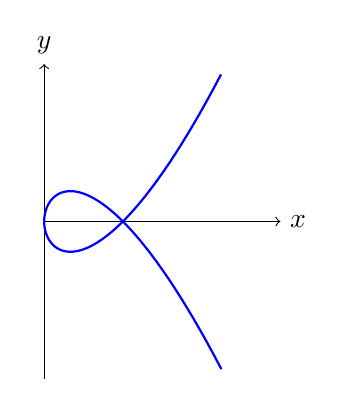
\begin{tikzpicture}
			\draw[->] (0,0) -- (3,0);
			\node[right] at (3,0) {$x$};
			\draw[->] (0,-2) -- (0,2);
			\node[above] at (0,2) {$y$};
			
			\draw[blue,thick,domain=-1.5:1.5,samples=100] plot ({\x*\x}, {\x*(\x*\x-1)});
		\end{tikzpicture}
		\end{center}
\end{enumerate}








\clearpage





{\bf Key Points to Remember:}

\vspace{5mm}

\begin{enumerate}
	\item A \textbf{parametrisation} of a curve $C$ is a pair of functions $x(t)$ and $y(t)$ and two times, $a$ and $b$, such that the point $(x(t),y(t))$ traces out the curve $C$ as $t$ varies from $a$ to $b$---\textit{i.e.}, it is instructions for a walk along $C$. The variable $t$ is called the \textbf{parameter}.
	\item The arc length $s$ of a parametrised curve is given by
		\begin{align*}
			s&=\int_a^b \sqrt{\left(\deriv{x}{t}\right)^2+\left(\deriv{y}{t}\right)^2}\diff t\\
			&=\int_{x(a)}^{x(b)}\sqrt{1+\left(\deriv{y}{x}\right)^2}\diff x\\
			&=\int_{y(a)}^{y(b)}\sqrt{\left(\deriv{x}{y}\right)^2+1}\diff y.
		\end{align*}
\end{enumerate}









\end{document}